\section{Actor-Critic with Experience Replay (ACER)}
\raggedbottom 

"Actor critic with experience replay" (ACER) introduced by \citet{ACER} was one of the first approaches to create a sample efficient, yet stable actor critic method, that applies to both contiuous and discrete action spaces.

ACER combines recent breakthroughs in the field of RL, by utilizing both the ressource efficient parallel training of RL agents proposed by \citet{A3C} and the Retrace algorithm \citep{Munos16}.

These approaches were combined with truncated importance sampling with bias correction and an efficient trust region policy optimization.
For continuous action spaces, stochastic dueling network architectures were used.

Acer can be viewed as an off-policy extension of A3C \citep{A3C}.

The importance weighted policy gradient is given by:
\begin{align}
\hat{g}^{imp} = \left(\prod^k_{t=0}p_t\right) \sum^k_{t=0}\left(\sum^k_{i=0}\gamma^ir_{t+i}\right) \nabla_\theta \ log \ \pi (a_t \mid s_t)
\end{align}

The unbounded importance weights can cause massive variance. \citet{Degris12} approached this problem by approximating the policy gradient as

\begin{align}
g^{marg} = E_{s_{t \textasciitilde{}} \beta, a_{t \textasciitilde{}} \mu} \left[p_t \nabla_\theta log \pi_\theta(a_t \mid s_t) Q^\pi (s_t,a_t) \left]
\end{align}

where $\beta$ denotes the limiting distribution and behaviour policy $\mu$

To compute this gradient, knowledge about $Q^\pi$ is nessecary. The retrace values (\ref{qretrace}) present a good estimation for $Q^\pi$.

To further reduce the variance, the importance weights are truncated.
A core problem of actor-critic methods is the tradeoff between bias and variance. By truncating the importance weights, bias is introduced.
To counter this, ACER uses a bias correction term.

The final ACER policy gradient is given as:

\begin{equation}
\begin{split}
g^{ACER}_t = \tilde{p}_t \nabla_\theta log \pi_\theta(a_t \mid s_t) \left[Q^{ret}(s_t,a_t) - V_\theta_v(s_t)\right] \\
+ E_{a_{\textasciitilde{}\pi}} \left(\left[\frac{p_t(a) -c}{p_t(a)\right]}_+ \nabla_\theta log \pi_\theta(a \mid s_t) \left[Q_\theta_v(s_t,a) - V_\theta_v(s_t)\right]\right)
\end{split}
\end{equation}

The critic $Q_\theta_v$ is trained by minimizing the mean squared error with the retrace values as the target.

\citet{ACER} proposed an efficient trust region policy optimization (TRPO), which limits the update step in a way, that the new policy doesnt deviate too much from an average policy. 
\pagebreak

Even though the improvement through the TRPO method on the continuous action space environments was significant, the results presented in the paper only showed a marginal improvement for discrete action space environments.
Because all experiments in this thesis are on discrete action space in order to run more experiments the TRPO was not used.

\subsection{Experimental Setup}

\subsubsection{Environment}
All experiments were made using multiple selected games from the Atari 2600 console game environments providede by \citet{openaigym}.

In our experiments the following OpenAI-Gym environments were used:

\textbf{Breakout} is a game that rapidly speeds up, making it easy for machines to show "superhuman" performance.

\textbf{Seaquest} poses a serious problem for learning agent, as they tend to get stuck on local maxima. It is especially interesting, as it provides multiple possibilities to achieve rewards, and the loss of the game if the player runs out of oxygen is a game mechanic a human can grasp in seconds, while it is notoriously hard for reinforcement learning agents to 'understand'.

Scoring well on this environment can be considered a great achievement.

\textbf{Space Invaders} is a fast paced game. Human and reinforcement learning approaches usually have similar scores. \citep{mnih2015atari}

The hyperparameters were adjusted to ensure a good performance for the Breakout environment. Test on other environments were all performed with the same set of hyperparameters.


OpenAI gym environments provide the agent with a 210x160 pixel colored image. An \textit{environment step} consist of frame skipping, which means, that the action fed into the environment is repeated for k frames. Where k denotes a random number within $\{2,3,4\}$.
\subsubsection{Preprocessing}
Using full scale colored images would come with huge computational cost. To be able to work with the data, each frame is preprocessed.
After grayscaling and transforming the frame, the scoreboard area is chopped off. With this method a 84x84 grayscaled pixel image is obtained. 

\citet{nature} proposed to stack multiple frames. More specifically the state contains the last 4 frames received and therefore has a shape of 84x84x4.

To receive the initial state, we simply stack the first frame 4 times.

\begin{figure}
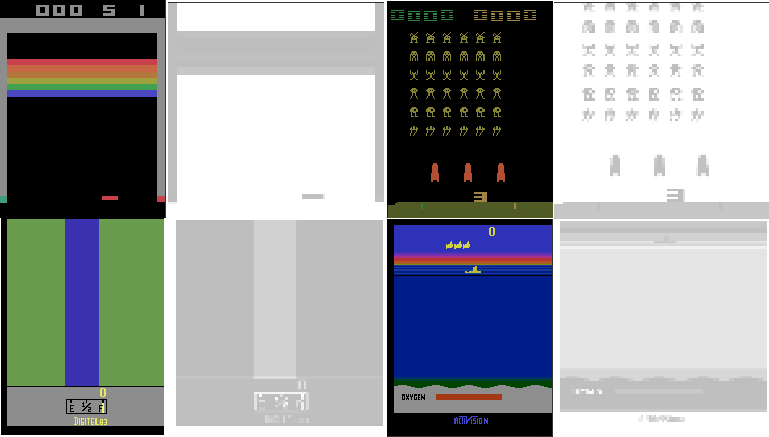
\includegraphics[scale=0.5]{bilder/atarienv.png}
\caption{The Atari 2600 console games Breakout, SpaceInvaders, Riverraid and Seaquest before and after being processed.}
\end{figure}

\subsubsection{network architecture}

Two architectures were tested. \citep{mnih2015atari} \citep{nature}.

Both provided good results. Since the paper uses the architecture proposed in the nature paper \citep{nature}, all further experiments were done using this architecture.

Similar to the \citep{A3C} network, most of the parameters are shared and used for both estimating $Q^\pi$ and to output a policy.

The shared net consists of 3 convolutional layers.
First 32 8x8 filters are applied with a stride of 4.
The 2nd layer consists of 64 4x4 filters using a stride of 2.
The last convolutional layer uses 64 3x3 filters with stride 1.
Finally a fully connected layer of size 512 is applied.

Each of the mentioned layers is followed by a rectifier nonlinearity (ReLU) function, ReLU is used to set all negative outputs to 0, ensuring only positive values are passed to the next layer.
Even though other activation/transformation functions exist, the ReLU has empirically done really well. 

A test run using tanh instead of ReLU caused a strong loss of performance.

The final shared layers is then mapped to the action space twice to obtain the action scores, and the Q-values. We use a softmax policy to receive the distribution over actions.
The action is randomly sampled from the softmax probabilities.

\begin{equation}
P(A = a' | s ) = \frac{e^{z_{a'}}}{\sum^N_{i=0}e^{z_{a_i}}} 
\end{equation}

where $z_{a}$ denotes the score assigned to the action through the last network layer.


\begin{figure}
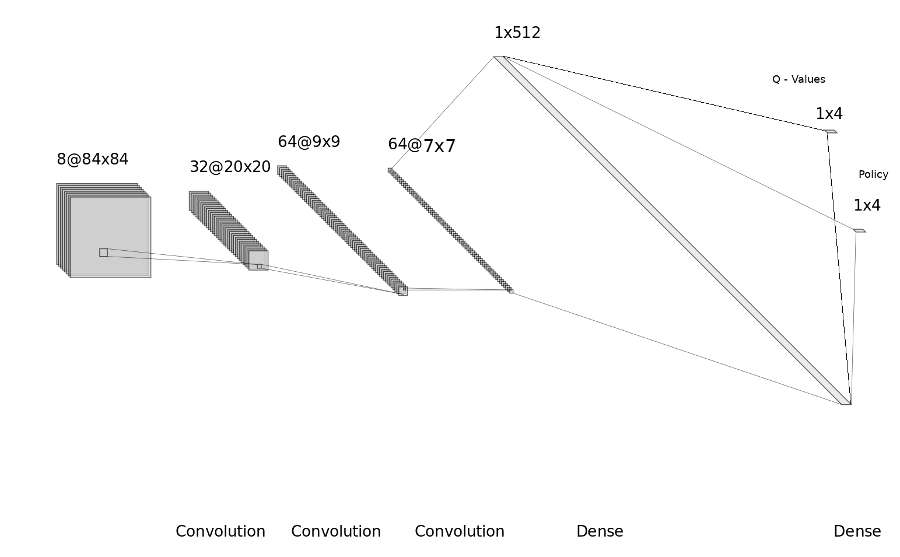
\includegraphics[scale=0.5]{bilder/nn2.png}
\caption{Shared network for policy and Q-Value approximization for an environment with 4 possible actions}
\end{figure}

The agent is trained by using 16 learner threads running on the CPU. Each Thread has it's own replay buffer, which ensures a more balanced replay and reduces the risk of a single trajectory being used unreasonably often compared to a single shared replay buffer.

Updates to the network were performed every 20 steps or if the environment reached a terminal state. 

Replay buffers were designed to hold up to 2500 trajectories, therefore ~50.000 frames were saved for each thread and $_\tilde{}$ 800.000 frames were stored in total, which is the same size used by DQN \citep{nature}}

If no replay is used, ACER essentially becomes a version of A3C which uses retrace and Q-values, rather than learning the value function. \citep{A3C}

For the offline setting, replay ratios of 1,2 and 4 were considered, where a ratio of 4 would mean, that the net is trained on trajectories sampled from the replay buffer 4 times for every online update.


